% =====================================================================
%  Software Requirements Specification (SRS) v1.0
%  Project : Higher Studies Tracking System
%  Team    : T070
%  Course  : CS314 -- Software Development Laboratory
%  Faculty : Dr. Saurabh Kumar
%  Inst.   : The LNM Institute of Information Technology, Jaipur
% =====================================================================
\documentclass[11pt,a4paper]{article}

% --- Geometry ---
\usepackage[a4paper,margin=2.2cm,top=2.2cm,bottom=2.2cm]{geometry}

% --- Encoding ---
\usepackage[T1]{fontenc}
\usepackage{lmodern}
\usepackage[utf8]{inputenc}

% --- Microtypography ---
\usepackage{microtype}

% --- Colour ---
\usepackage[dvipsnames]{xcolor}
\definecolor{primary}{HTML}{1F4E79}
\definecolor{accent}{HTML}{2E75B6}

% --- Tables ---
\usepackage{booktabs}
\usepackage{longtable}
\usepackage{tabularx}
\usepackage{array}
\usepackage{makecell}
\renewcommand{\arraystretch}{1.05}
\newcolumntype{Y}{>{\raggedright\arraybackslash}X}

% --- Lists ---
\usepackage{enumitem}
\setlist{nosep,leftmargin=*}

% --- Page layout: no inter-paragraph skip, ragged bottom (no stretch) ---
\setlength{\parskip}{0pt}
\setlength{\parindent}{0pt}
\raggedbottom

% --- Sectioning ---
\usepackage{titlesec}
\titleformat{\section}{\Large\bfseries\color{primary}}{\thesection}{0.8em}{}
\titleformat{\subsection}{\large\bfseries\color{primary}}{\thesubsection}{0.6em}{}
\titleformat{\subsubsection}{\normalsize\bfseries\color{accent}}{\thesubsubsection}{0.5em}{}
\titlespacing*{\section}{0pt}{1.2em}{0.5em}
\titlespacing*{\subsection}{0pt}{0.8em}{0.3em}
\titlespacing*{\subsubsection}{0pt}{0.6em}{0.2em}

% --- TikZ ---
\usepackage{tikz}
\usetikzlibrary{shapes.geometric, arrows.meta, positioning, fit, backgrounds, calc}

% --- Hyperref ---
\usepackage{hyperref}
\hypersetup{
  colorlinks=true,
  linkcolor=primary,
  urlcolor=primary,
  citecolor=primary,
  pdftitle={SRS v1.0 -- Higher Studies Tracking System},
  pdfauthor={Team T070}
}

% --- Captions (proper full-width captions above tables) ---
\usepackage{caption}
\captionsetup{labelfont=bf, labelsep=period, position=top, skip=4pt, font=small}

% --- Title block ---
\title{
  {\Huge\bfseries\color{primary} Software Requirements Specification}\\[6pt]
  {\LARGE\bfseries Version 1.0}\\[8pt]
  {\Large\itshape Higher Studies Tracking System}\\[10pt]
  \rule{\textwidth}{0.4pt}\\[6pt]
  {\normalsize CS314 -- Software Development Laboratory}\\
  {\normalsize The LNM Institute of Information Technology, Jaipur}\\[2pt]
  {\normalsize Faculty: Dr. Saurabh Kumar}
}
\author{}
\date{}

% =====================================================================
\begin{document}
\maketitle
\vspace{-0.5cm}
\begin{center}
\small\itshape
Prepared by Team T070\par
LAXITA BHIMSARIA (24UCS144, Project/Requirement Lead) \quad
VAIBHAV GOYAL (24UCS145, Design/Architecture Lead)\\
MANAN JAIN (24UCS146, Development Lead) \quad
HARSH VARSHNEY (24UCS148, Testing \& Documentation Lead)\par
\end{center}
\vspace{0.4cm}

\pdfbookmark[0]{Contents}{toc}
\tableofcontents
\newpage

% =====================================================================
\section*{Document Control}
\addcontentsline{toc}{section}{Document Control}
\begin{tabularx}{\textwidth}{@{}l Y l Y@{}}
\toprule
\textbf{Version} & \textbf{Description} & \textbf{Date} & \textbf{Author} \\
\midrule
1.0 & Initial baseline SRS for the Higher Studies Tracking System,
 derived from Assignment~1 (Project Identification, 31~Aug~2026). & 2026-08-31 & Team T070 \\
\bottomrule
\end{tabularx}

\section{Introduction}
\subsection{Purpose}
This Software Requirements Specification (SRS) defines the functional and
non-functional requirements of the \emph{Higher Studies Tracking System}
(HSTS), a web-based application developed by Team~T070 as part of
CS314 (Software Development Laboratory) at LNMIIT Jaipur. It is the
baseline document that will drive subsequent UML analysis, design,
implementation and testing activities.

\subsection{Product Scope}
HSTS centralises the recording, verification and tracking of higher-study
information for graduating students and alumni of the institute. It
supports role-based workflows for students/alumni, higher studies
coordinators, administrators and authorised faculty, and provides basic
search, filtering and reporting facilities. Out-of-scope items (such as
university application submission, fee processing, visa processing and
alumni networking) are explicitly listed in the Assignment~1 brief and
are excluded from this release.

\subsection{Definitions, Acronyms, Abbreviations}
\begin{itemize}
  \item \textbf{SRS} -- Software Requirements Specification.
  \item \textbf{FR / BR / NFR} -- Functional Requirement / Business Rule /
 Non-Functional Requirement.
  \item \textbf{UC / US / AC} -- Use Case / User Story / Acceptance Criterion.
  \item \textbf{RTM} -- Requirements Traceability Matrix.
  \item \textbf{MoSCoW} -- Must have / Should have / Could have / Won't have.
  \item \textbf{HSTS} -- Higher Studies Tracking System.
\end{itemize}

\subsection{References}
\begin{enumerate}
  \item CS314 Lab Assignment 1 -- Project Identification and Initial Project Definition (Team T070, 31~Aug~2026).
  \item CS314 Lab Assignment 2 -- Requirements Specification brief.
  \item IEEE Std 830-1998 -- Recommended Practice for Software Requirements
        Specifications.
  \item CS314 Project Guidelines for Students (course handbook).
\end{enumerate}

\subsection{Document Overview}
Section~1 lists user classes and the system context. Sections~3--6
define the functional, business-rule, non-functional and data
requirements. Sections~7--9 document the use cases, user stories and
acceptance criteria. Sections~10--13 cover MoSCoW prioritisation,
traceability and a self-administered validation review.

% =====================================================================
\section{User Classes}
The user classes below are derived from the stakeholder analysis in
Assignment~1, Section~6. Each class is briefly described together with
its main interactions with HSTS.

\subsection*{UC-1.1 Student / Alumni}
The primary data contributor. Creates, maintains and views their own
higher-study record; updates admission status; receives notifications
related to their own records.

\subsection*{UC-1.2 Higher Studies Coordinator}
The verifier and day-to-day operator. Searches and filters records;
verifies or rejects student-submitted records (with reasons); records
progression updates; generates status, institution and programme reports.

\subsection*{UC-1.3 Administrator}
Manages user accounts and role assignments; monitors audit logs;
configures system-level reference data (institutions, programmes,
countries); accesses administrative reports.

\subsection*{UC-1.4 Institute Management / Authorised Faculty}
Read-only consumer of aggregated reports and dashboards for academic
planning and outcome reporting.

% =====================================================================
\section{System Context}
The system context diagram below shows HSTS as a single bounded system
interacting with its four primary user classes and one external service
(the e-mail/notification service used for outbound messages).

\begin{figure}[h!]
\centering
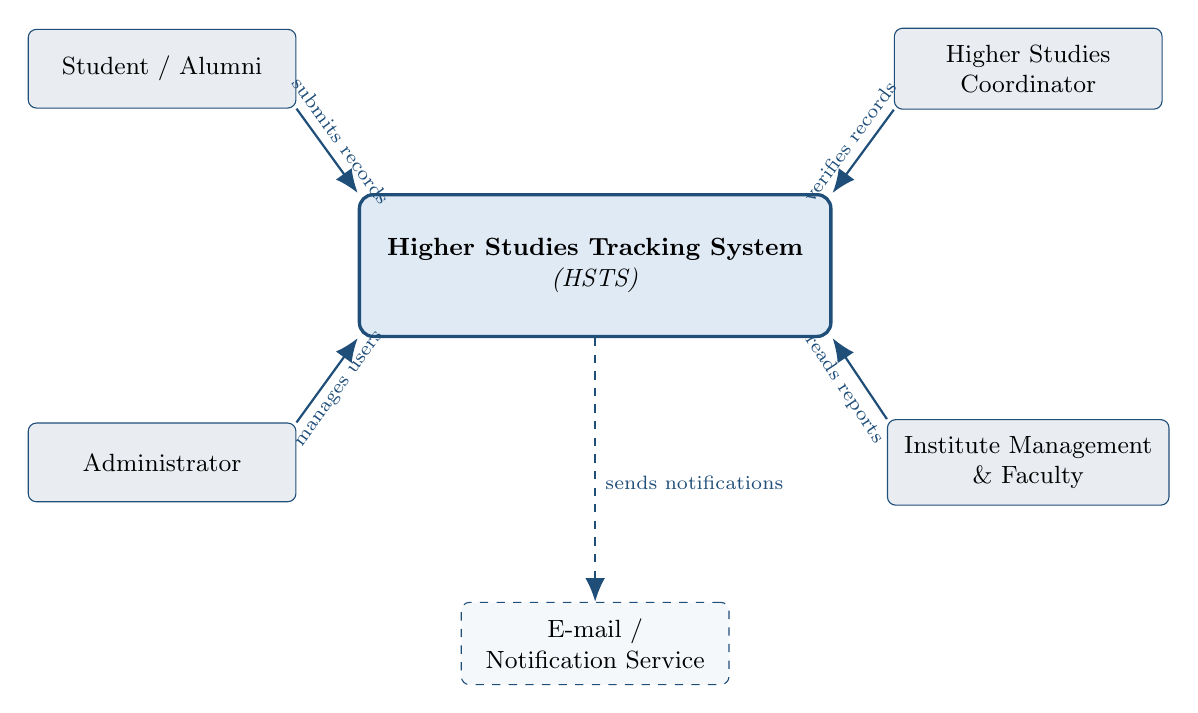
\begin{tikzpicture}[
    every node/.style={font=\small},
    actor/.style={
        rectangle, rounded corners=3pt,
        draw=primary, fill=primary!10,
        minimum width=3.4cm, minimum height=1cm,
        align=center, inner sep=6pt
    },
    system/.style={
        rectangle, rounded corners=5pt,
        draw=primary, very thick,
        fill=accent!15,
        minimum width=4.8cm, minimum height=1.8cm,
        align=center, inner sep=10pt
    },
    ext/.style={
        rectangle, rounded corners=3pt,
        draw=primary, fill=accent!5, dashed,
        minimum width=3.4cm, minimum height=1cm,
        align=center, inner sep=6pt
    },
    arrow/.style={-{Latex[length=3mm,width=2.5mm]}, thick, primary}
]
% System at the centre
\node[system] (sys) at (0, 0) {%
    \textbf{Higher Studies Tracking System}\\
    \textit{(HSTS)}
};

% Actors at the four corners around the system
\node[actor] (stu) at (-5.5, 2.5)  {Student / Alumni};
\node[actor] (coo) at ( 5.5, 2.5)  {Higher Studies\\Coordinator};
\node[actor] (adm) at (-5.5,-2.5) {Administrator};
\node[actor] (mgm) at ( 5.5,-2.5) {Institute Management\\ \& Faculty};

% External entity below the system
\node[ext]   (mail) at (0, -4.8) {E-mail /\\Notification Service};

% Arrows: each actor connects to the system
\draw[arrow] (stu.south east) -- node[above, sloped, font=\scriptsize]{submits records} (sys.north west);
\draw[arrow] (coo.south west) -- node[above, sloped, font=\scriptsize]{verifies records} (sys.north east);
\draw[arrow] (adm.north east) -- node[below, sloped, font=\scriptsize]{manages users} (sys.south west);
\draw[arrow] (mgm.north west) -- node[below, sloped, font=\scriptsize]{reads reports} (sys.south east);

% Arrow from system to external entity (vertical, no overlap with corner actors)
\draw[arrow, dashed] (sys.south) -- node[right, font=\scriptsize, pos=0.55]{sends notifications} (mail.north);
\end{tikzpicture}
\caption{Context-level diagram of the Higher Studies Tracking System.}
\label{fig:context}
\end{figure}

\noindent\textbf{Notes:}
\begin{itemize}
  \item All four user classes authenticate before interacting with HSTS.
  \item The e-mail/notification service is an external dependency used for outbound messages only; HSTS does not depend on it for core database operations.
  \item Students/Alumni do not have direct access to other students' records.
\end{itemize}

% =====================================================================
\section{Functional Requirements}
All functional requirements are written in the form \emph{``The system
shall\ldots''}. Each FR has a unique identifier (FR-NNN), a short title,
the full requirement text, and (where relevant) a reference to a related
business rule in Section~4.

\subsection{Authentication and Account Management}
\begin{tabularx}{\textwidth}{@{}p{1.6cm} p{4.0cm} Y@{}}
\caption{Functional requirements -- Authentication and Account Management.}
\label{tab:fr-auth}
\toprule
\textbf{ID} & \textbf{Title} & \textbf{Requirement} \\
\midrule
FR-001 & User Registration &
  The system shall allow a Student/Alumni to register an account using a valid institutional e-mail address and a self-chosen password. \\
FR-002 & User Login &
  The system shall allow a registered user to authenticate using valid credentials. \\
FR-003 & Authentication Failure Notification &
  The system shall notify the user when authentication fails without revealing which of the credentials was incorrect. \\
FR-004 & Logout &
  The system shall allow an authenticated user to terminate their session. \\
FR-005 & Role Assignment &
  The system shall allow an Administrator to assign one or more roles to a user account. \\
FR-006 & Role-Based Access Control &
  The system shall restrict access to functions according to the role(s) assigned to the authenticated user. \\
\bottomrule
\end{tabularx}

\subsection{Higher-Study Profile Management}
\begin{tabularx}{\textwidth}{@{}p{1.6cm} p{4.0cm} Y@{}}
\caption{Functional requirements -- Higher-Study Profile Management.}
\label{tab:fr-profile}
\toprule
\textbf{ID} & \textbf{Title} & \textbf{Requirement} \\
\midrule
FR-007 & Create Higher-Study Record &
  The system shall allow an authenticated Student/Alumni to create a higher-study record capturing institution, programme, country, applied intake year and any additional declared information. \\
FR-008 & Edit Higher-Study Record &
  The system shall allow an authenticated Student/Alumni to edit their own record while it is in \emph{Draft} or \emph{Rejected} status. \\
FR-009 & View Higher-Study Record &
  The system shall allow a Student/Alumni to view all of their own higher-study records together with current status and history. \\
FR-010 & Manage Institution Records &
  The system shall allow an Administrator to maintain the list of institutions that can be referenced in higher-study records. \\
FR-011 & Manage Programme Records &
  The system shall allow an Administrator to maintain the list of programmes (degree, field of study) that can be referenced in higher-study records. \\
FR-012 & Manage Country Records &
  The system shall allow an Administrator to maintain the list of countries that can be referenced in higher-study records. \\
FR-013 & Multiple Applications &
  The system shall allow a Student/Alumni to maintain more than one higher-study record concurrently (e.g.\ multiple applications). \\
FR-014 & Deactivate Record &
  The system shall allow an authorised user to deactivate a record in place of permanent deletion (see BR-006). \\
\bottomrule
\end{tabularx}

\subsection{Admission and Progression Status}
\begin{tabularx}{\textwidth}{@{}p{1.6cm} p{4.0cm} Y@{}}
\caption{Functional requirements -- Admission and Progression Status.}
\label{tab:fr-status}
\toprule
\textbf{ID} & \textbf{Title} & \textbf{Requirement} \\
\midrule
FR-015 & Set Admission Status &
  The system shall allow a Student/Alumni to set the admission status of their record to \emph{Applied} when first creating it, and to subsequently update it through the lifecycle defined in BR-002. \\
FR-016 & Status Transition Validation &
  The system shall reject any status change that does not conform to the allowed lifecycle in BR-002 and shall display an explanatory message. \\
FR-017 & Record Progression Updates &
  The system shall allow an authorised Coordinator to record progression updates (e.g.\ coursework completed, thesis submitted) against an enrolled record. \\
FR-018 & View Status History &
  The system shall display the complete chronological status and progression history for each higher-study record, including the user responsible for each change and the timestamp. \\
FR-019 & Final Outcome Capture &
  The system shall allow an authorised Coordinator to record the final outcome of a record as \emph{Completed} or \emph{Withdrawn}. \\
\bottomrule
\end{tabularx}

\subsection{Verification Workflow}
\begin{tabularx}{\textwidth}{@{}p{1.6cm} p{4.0cm} Y@{}}
\caption{Functional requirements -- Verification Workflow.}
\label{tab:fr-verify}
\toprule
\textbf{ID} & \textbf{Title} & \textbf{Requirement} \\
\midrule
FR-020 & Verify Record &
  The system shall allow an authorised Higher Studies Coordinator to mark a submitted record as \emph{Verified}. \\
FR-021 & Reject Verification with Reason &
  The system shall allow an authorised Higher Studies Coordinator to reject a submitted record, requiring a textual reason. \\
FR-022 & Add Verification Comment &
  The system shall allow a Coordinator to attach free-text comments to a verification decision. \\
FR-023 & View Verification History &
  The system shall display the complete verification history (verifier, decision, reason, comments, timestamp) for each record. \\
\bottomrule
\end{tabularx}

\subsection{Search, Filter and Listing}
\begin{tabularx}{\textwidth}{@{}p{1.6cm} p{4.0cm} Y@{}}
\caption{Functional requirements -- Search, Filter and Listing.}
\label{tab:fr-search}
\toprule
\textbf{ID} & \textbf{Title} & \textbf{Requirement} \\
\midrule
FR-024 & List Records &
  The system shall allow a Coordinator or Administrator to list higher-study records with pagination. \\
FR-025 & Free-Text Search &
  The system shall allow a Coordinator or Administrator to search records by student name, roll number or institution. \\
FR-026 & Filter by Institution &
  The system shall allow records to be filtered by institution. \\
FR-027 & Filter by Country &
  The system shall allow records to be filtered by country. \\
FR-028 & Filter by Status &
  The system shall allow records to be filtered by admission or verification status. \\
\bottomrule
\end{tabularx}

\subsection{Reports and Dashboard}
\begin{tabularx}{\textwidth}{@{}p{1.6cm} p{4.0cm} Y@{}}
\caption{Functional requirements -- Reports and Dashboard.}
\label{tab:fr-reports}
\toprule
\textbf{ID} & \textbf{Title} & \textbf{Requirement} \\
\midrule
FR-029 & Status Distribution Report &
  The system shall generate a report showing the distribution of records across admission statuses. \\
FR-030 & Institution-Wise Report &
  The system shall generate a report aggregating record counts by institution. \\
FR-031 & Country-Wise Report &
  The system shall generate a report aggregating record counts by country. \\
FR-032 & Programme-Wise Report &
  The system shall generate a report aggregating record counts by programme. \\
FR-033 & Administrative Dashboard &
  The system shall provide an Administrative dashboard summarising key counts (total records, pending verifications, recent verifications). \\
\bottomrule
\end{tabularx}

% =====================================================================
\section{Business Rules}
\begin{tabularx}{\textwidth}{@{}p{1.4cm} p{5.2cm} Y@{}}
\caption{Business rules.}
\label{tab:br}
\toprule
\textbf{ID} & \textbf{Title} & \textbf{Rule} \\
\midrule
BR-001 & Self-Service Records &
  A Student/Alumni may create, edit and submit only their own higher-study records. \\
BR-002 & Admission Status Lifecycle &
  Admission status shall follow the lifecycle \emph{Applied $\rightarrow$ (Accepted $\mid$ Rejected) $\rightarrow$ Enrolled \ $\rightarrow$ (Completed $\mid$ Withdrawn)}. Transitions outside this lifecycle are rejected by the system. \\
BR-003 & Coordinator Verification Authority &
  Only a user holding the \emph{Higher Studies Coordinator} role may verify or reject a record. \\
BR-004 & Edit Lock After Verification &
  Once a record has been verified, only a Coordinator may edit it; a Student/Alumni may no longer modify it directly. \\
BR-005 & Rejection Reason Mandatory &
  A verification rejection shall not be saved without a textual reason. \\
BR-006 & No Hard Delete (Soft Deactivation) &
  Higher-study records shall not be permanently deleted; deactivation shall preserve the full historical record for auditing. \\
BR-007 & Multiple Concurrent Applications &
  A Student/Alumni may hold more than one active record simultaneously, reflecting multiple parallel applications. \\
BR-008 & Audit Attribution &
  Every status change, verification decision and edit to a record shall be attributed to a user and timestamped in the status history. \\
BR-009 & Self-Access Only for Students &
  A Student/Alumni may view only their own records; viewing other students' records is denied. \\
BR-010 & Reports Use Verified Data First &
  Aggregate reports shall be computed over verified records by default; unverified records shall be reported separately when included. \\
\bottomrule
\end{tabularx}

% =====================================================================
\section{Non-Functional Requirements}

\subsection{Performance}
\begin{itemize}
  \item \textbf{NFR-001} The system shall return responses to typical user operations (page loads, form submissions, record lookups) within 2~seconds under expected concurrent load.
  \item \textbf{NFR-002} Free-text search across higher-study records (FR-025) shall return results within 3~seconds for the expected data volume.
  \item \textbf{NFR-003} The system shall support at least 50~concurrent authenticated users without degradation beyond the targets in NFR-001 and NFR-002.
\end{itemize}

\subsection{Security}
\begin{itemize}
  \item \textbf{NFR-004} Passwords shall be stored using a strong adaptive cryptographic hash (e.g.\ bcrypt/Argon2) and shall never be logged or transmitted in clear text.
  \item \textbf{NFR-005} All access to protected resources shall require a successful authentication.
  \item \textbf{NFR-006} Role-based authorisation shall be enforced at every API endpoint in addition to any UI-level checks.
  \item \textbf{NFR-007} The system shall protect against common web vulnerabilities including SQL injection, XSS and CSRF.
\end{itemize}

\subsection{Usability}
\begin{itemize}
  \item \textbf{NFR-008} The interface shall provide consistent navigation across all major user-facing pages.
  \item \textbf{NFR-009} Form validation errors shall be presented in human-readable language next to the offending field.
  \item \textbf{NFR-010} The most common task for each user role shall be reachable within two navigation steps from the dashboard.
\end{itemize}

\subsection{Reliability}
\begin{itemize}
  \item \textbf{NFR-011} Status and verification data shall be persisted within an atomic transaction; partial failures shall not leave a record in an inconsistent state.
  \item \textbf{NFR-012} Database backups shall be performed daily and a documented restore procedure shall be available.
\end{itemize}

\subsection{Availability}
\begin{itemize}
  \item \textbf{NFR-013} The system shall target 99\% availability during normal institute operating hours, excluding scheduled maintenance windows communicated in advance.
\end{itemize}

\subsection{Maintainability}
\begin{itemize}
  \item \textbf{NFR-014} The application shall be organised into clearly separated modules (presentation, application logic, data access) to enable independent modification.
  \item \textbf{NFR-015} Source code shall be maintained in a Git repository with meaningful, atomic commits.
  \item \textbf{NFR-016} Technical and user documentation shall be updated in the same commit that changes the corresponding behaviour.
\end{itemize}

\subsection{Scalability}
\begin{itemize}
  \item \textbf{NFR-017} The application tier shall be horizontally scalable through stateless request handling.
  \item \textbf{NFR-018} Database schema shall include indexes on the most common search and filter columns (institution, country, status, student identifier).
\end{itemize}

\subsection{Privacy}
\begin{itemize}
  \item \textbf{NFR-019} Personal information of students shall be accessible only to authorised users and shall not be exposed in public reports.
  \item \textbf{NFR-020} Personally identifying fields shall be masked in administrative listings shown to users without view-on-record permission.
\end{itemize}

\subsection{Compatibility}
\begin{itemize}
  \item \textbf{NFR-021} The system shall operate correctly on the current major versions of Chrome, Firefox, Edge and Safari.
\end{itemize}

\subsection{Auditability}
\begin{itemize}
  \item \textbf{NFR-022} Significant actions (status changes, verification decisions, user/role management, deactivation) shall be written to an append-only audit log including user, timestamp, action and target record.
  \item \textbf{NFR-023} Audit log entries shall be retained for a minimum of one academic year and shall be viewable by Administrators.
\end{itemize}

% =====================================================================
\section{Data Requirements}
The following logical entities are required to support the functional
requirements in Section~3 and the business rules in Section~4. Attribute
lists are non-exhaustive and represent the most important fields.

\begin{longtable}{@{}p{3.6cm} p{4.0cm} p{8.0cm}@{}}
\caption{Major data entities and their key attributes.}
\label{tab:data}
\toprule
\textbf{Entity} & \textbf{Key Attributes} & \textbf{Notes} \\
\midrule
\endfirsthead
\toprule
\textbf{Entity} & \textbf{Key Attributes} & \textbf{Notes} \\
\midrule
\endhead
User & user\_id, name, email, password\_hash, status, created\_at & Identity record for every system actor. \\
Role & role\_id, name, description & Reference data; supports the RBAC model in FR-006. \\
UserRole & user\_id, role\_id & Join entity linking users to their assigned roles. \\
Student & student\_id, roll\_no, name, programme\_of\_study, batch\_year & Derived from institute records; subject to BR-009 access rules. \\
Institution & institution\_id, name, country, type & Reference data maintained by Administrators. \\
Programme & programme\_id, name, level (UG/PG/PhD), field\_of\_study & Reference data maintained by Administrators. \\
Country & country\_id, name, code & Reference data maintained by Administrators. \\
HigherStudyRecord & record\_id, student\_id, institution\_id, programme\_id, country\_id, intake\_year, admission\_status, verification\_status, is\_active, created\_at, updated\_at & Central entity; subject to BR-002, BR-004, BR-006. \\
AdmissionStatusHistory & history\_id, record\_id, from\_status, to\_status, changed\_by, changed\_at, reason & Implements BR-008; supports FR-018. \\
VerificationRecord & verification\_id, record\_id, decision, reason, comments, verified\_by, verified\_at & Implements FR-020--FR-023 and BR-005. \\
AuditLog & log\_id, user\_id, action, target\_type, target\_id, timestamp, details & Implements NFR-022 / NFR-023; append-only. \\
\bottomrule
\end{longtable}

% =====================================================================
\section{Major Use Cases}
\begin{longtable}{@{}p{1.4cm} p{6.5cm} p{8.0cm}@{}}
\caption{Major use cases and their primary actors.}
\label{tab:uc}
\toprule
\textbf{ID} & \textbf{Use Case} & \textbf{Primary Actor} \\
\midrule
\endfirsthead
\toprule
\textbf{ID} & \textbf{Use Case} & \textbf{Primary Actor} \\
\midrule
\endhead
UC-001 & Register User Account & Student / Alumni \\
UC-002 & Log In & All Users \\
UC-003 & Manage User Accounts and Roles & Administrator \\
UC-004 & Create Higher-Study Record & Student / Alumni \\
UC-005 & Edit Higher-Study Record & Student / Alumni \\
UC-006 & Update Admission Status & Student / Alumni \\
UC-007 & Verify Higher-Study Record & Higher Studies Coordinator \\
UC-008 & Reject Higher-Study Record & Higher Studies Coordinator \\
UC-009 & View Status and Verification History & Student / Alumni \\
UC-010 & Search Higher-Study Records & Higher Studies Coordinator \\
UC-011 & Filter Higher-Study Records & Higher Studies Coordinator \\
UC-012 & Generate Status Distribution Report & Higher Studies Coordinator \\
UC-013 & Generate Institution / Country / Programme Reports & Higher Studies Coordinator \\
UC-014 & View Administrative Dashboard & Administrator \\
UC-015 & View Audit Log & Administrator \\
\bottomrule
\end{longtable}

% =====================================================================
\section{Detailed Use Cases}
Three use cases considered most critical are elaborated below.

\subsection{UC-004 -- Create Higher-Study Record}

\noindent\textbf{Primary Actor:} Student / Alumni.

\medskip

\noindent\textbf{Goal:} Capture a new higher-study application in the system.

\medskip

\noindent\textbf{Preconditions:}
\begin{itemize}
  \item The user is authenticated (FR-002).
  \item The student profile is linked to the authenticated user.
  \item The targeted institution, programme and country exist as reference data (FR-010--FR-012).
\end{itemize}

\medskip

\noindent\textbf{Main Flow:}
\begin{enumerate}
  \item Student selects \emph{Add Higher-Study Record}.
  \item System presents an empty form with institution, programme, country, intake year and notes fields.
  \item Student enters the data and submits the form.
  \item System validates the inputs against reference data and mandatory-field rules.
  \item System persists the record with admission status \emph{Applied} (BR-002) and verification status \emph{Pending}.
  \item System confirms successful creation and displays the new record in the student's profile.
\end{enumerate}

\medskip

\noindent\textbf{Alternative / Exception Flows:}
\begin{itemize}
  \item \emph{Invalid input}: system highlights offending fields with human-readable messages (NFR-009) and returns to step~3.
  \item \emph{Reference data missing}: system prevents submission and advises the user to contact the Administrator.
  \item \emph{Authentication lost}: system redirects to login (FR-002).
\end{itemize}

\medskip

\noindent\textbf{Postconditions:} A new higher-study record exists with status \emph{Applied} and is visible to the student and to Coordinators in pending lists.

\subsection{UC-007 -- Verify Higher-Study Record}

\noindent\textbf{Primary Actor:} Higher Studies Coordinator.

\medskip

\noindent\textbf{Goal:} Officially validate a submitted higher-study record.

\medskip

\noindent\textbf{Preconditions:}
\begin{itemize}
  \item The Coordinator is authenticated.
  \item At least one record exists in \emph{Pending} verification status.
\end{itemize}

\medskip

\noindent\textbf{Main Flow:}
\begin{enumerate}
  \item Coordinator opens the list of pending records (UC-010).
  \item Coordinator selects a record to review.
  \item System displays the record details, status history and student profile.
  \item Coordinator chooses \emph{Verify}.
  \item System records the verification decision with the Coordinator as verifier and the current timestamp (BR-008, FR-022).
  \item System updates the record's verification status to \emph{Verified} and confirms the action.
\end{enumerate}

\medskip

\noindent\textbf{Alternative / Exception Flows:}
\begin{itemize}
  \item \emph{Reject}: Coordinator chooses \emph{Reject}; system requires a textual reason (BR-005), records the rejection (FR-021) and returns the record to the student for correction.
  \item \emph{Add comment}: Coordinator optionally attaches a comment (FR-022) to either decision.
  \item \emph{Race condition}: if the record was modified by another user after retrieval, system refreshes the view and warns the Coordinator before allowing the decision to be saved.
\end{itemize}

\medskip

\noindent\textbf{Postconditions:} The record carries a permanent verification decision and is included in reports (BR-010).

\subsection{UC-012 -- Generate Status Distribution Report}

\noindent\textbf{Primary Actor:} Higher Studies Coordinator.

\medskip

\noindent\textbf{Goal:} Obtain an aggregated view of how records are distributed across admission statuses.

\medskip

\noindent\textbf{Preconditions:}
\begin{itemize}
  \item The Coordinator is authenticated.
  \item Sufficient data exists in the system to compute a meaningful distribution.
\end{itemize}

\medskip

\noindent\textbf{Main Flow:}
\begin{enumerate}
  \item Coordinator selects \emph{Reports $\rightarrow$ Status Distribution}.
  \item System offers filters for intake year, programme and country.
  \item Coordinator applies desired filters and confirms.
  \item System aggregates the matching records by admission status (FR-029), counting verified and unverified records separately (BR-010).
  \item System displays a table and a simple bar visualisation of the counts, with a timestamp and the applied filters.
  \item Coordinator optionally exports the report.
\end{enumerate}

\medskip

\noindent\textbf{Alternative / Exception Flows:}
\begin{itemize}
  \item \emph{No matching records}: system displays an empty-state message rather than failing.
  \item \emph{Filter conflict}: if a combination yields zero results, system suggests relaxing filters.
\end{itemize}

\medskip

\noindent\textbf{Postconditions:} The Coordinator has a status-distribution view corresponding to the chosen filters; the report is not stored as a separate record unless explicitly exported.

% =====================================================================
\section{User Stories}
\begin{longtable}{@{}p{1.4cm} p{14.5cm}@{}}
\caption{User stories derived from the requirements in Sections 3--6.}
\label{tab:us}
\toprule
\textbf{ID} & \textbf{Story} \\
\midrule
\endfirsthead
\toprule
\textbf{ID} & \textbf{Story} \\
\midrule
\endhead
US-001 & As a Student/Alumni, I want to register an account with my institute e-mail so that I can use the Higher Studies Tracking System. \\
US-002 & As a Student/Alumni, I want to log in securely so that I can access my own higher-study records. \\
US-003 & As a Student/Alumni, I want to create a higher-study record with my institution, programme and country so that my application is tracked centrally. \\
US-004 & As a Student/Alumni, I want to update my admission status as it changes so that my information remains accurate. \\
US-005 & As a Student/Alumni, I want to view the status and verification history of my records so that I know where each application stands. \\
US-006 & As a Higher Studies Coordinator, I want to verify a submitted record so that it becomes an official entry in the system. \\
US-007 & As a Higher Studies Coordinator, I want to reject a record with a reason so that the student can correct it. \\
US-008 & As a Higher Studies Coordinator, I want to search records by name, roll number or institution so that I can find specific applications quickly. \\
US-009 & As a Higher Studies Coordinator, I want to filter pending records so that I can process verifications efficiently. \\
US-010 & As a Higher Studies Coordinator, I want to generate a status distribution report so that I can summarise outcomes for the institute. \\
US-011 & As an Administrator, I want to manage user accounts and roles so that access to the system is controlled. \\
US-012 & As an Administrator, I want to maintain reference data (institutions, programmes, countries) so that records reference consistent values. \\
US-013 & As an Administrator, I want to view an audit log so that I can investigate changes to records and user accounts. \\
US-014 & As Institute Management, I want to view an aggregated dashboard so that I can understand higher-study outcomes for planning. \\
\bottomrule
\end{longtable}

% =====================================================================
\section{Acceptance Criteria}
Acceptance criteria are provided for three of the highest-priority user
stories. Each criterion is a single, testable, observable condition.

\subsection*{US-003 -- Create Higher-Study Record}
\begin{itemize}
  \item \textbf{AC-01} The user must be authenticated (FR-002) before the \emph{Add Higher-Study Record} option is offered.
  \item \textbf{AC-02} All mandatory fields (institution, programme, country, intake year) must be supplied; the system must display a clear, field-level error otherwise (NFR-009).
  \item \textbf{AC-03} The selected institution, programme and country must exist in the reference data maintained by the Administrator (FR-010--FR-012).
  \item \textbf{AC-04} On successful creation, the new record must appear in the student's profile with admission status \emph{Applied} (BR-002) and verification status \emph{Pending}.
  \item \textbf{AC-05} The new record must be visible in the Coordinator's pending-verification list (UC-007) within the same session.
\end{itemize}

\subsection*{US-006 -- Verify Higher-Study Record}
\begin{itemize}
  \item \textbf{AC-06} Only a user holding the Higher Studies Coordinator role may see the \emph{Verify} and \emph{Reject} actions (FR-006, BR-003).
  \item \textbf{AC-07} Selecting \emph{Verify} must mark the record as \emph{Verified} and must record the verifying Coordinator and a timestamp (BR-008, FR-022).
  \item \textbf{AC-08} Selecting \emph{Reject} must require a textual reason before saving (BR-005, FR-021).
  \item \textbf{AC-09} Once verified, the Student/Alumni must no longer be able to edit the record directly (BR-004).
  \item \textbf{AC-10} The verification decision must appear in the record's verification history (FR-023).
\end{itemize}

\subsection*{US-010 -- Generate Status Distribution Report}
\begin{itemize}
  \item \textbf{AC-11} The report must aggregate counts of records grouped by admission status (FR-029) and must clearly separate verified from unverified records (BR-010).
  \item \textbf{AC-12} The Coordinator must be able to filter the report by intake year, programme and country and the report must reflect the chosen filters.
  \item \textbf{AC-13} If no records match the filters, the system must display an empty-state message rather than an error.
  \item \textbf{AC-14} The report must display the timestamp of generation and the filter parameters applied.
\end{itemize}

% =====================================================================
\section{Requirements Prioritisation (MoSCoW)}

\subsection*{Must Have (Initial Release)}
\begin{itemize}
  \item Authentication and role-based access (FR-001--FR-006).
  \item Higher-study profile CRUD with multiple applications (FR-007--FR-009, FR-013).
  \item Admission status lifecycle and history (FR-015--FR-019, BR-002).
  \item Coordinator verification with reason and history (FR-020--FR-023, BR-003--BR-005).
  \item Reference data management by Administrator (FR-010--FR-012).
  \item Basic search, filter and listing (FR-024--FR-028).
  \item Status, institution, country and programme reports (FR-029--FR-032).
  \item Soft-deactivation instead of hard delete (FR-014, BR-006).
  \item Audit logging of significant actions (NFR-022, NFR-023).
\end{itemize}

\subsection*{Should Have}
\begin{itemize}
  \item Administrative dashboard (FR-033).
  \item Free-text comments on verification decisions (FR-022).
  \item Detailed verification history view (FR-023).
  \item Pagination on record lists (FR-024).
\end{itemize}

\subsection*{Could Have}
\begin{itemize}
  \item E-mail notifications on key events (e.g.\ status changes, verification decisions).
  \item Bulk actions for Coordinators (e.g.\ multi-record verification).
  \item Export of reports to CSV/PDF.
  \item Self-service password reset.
\end{itemize}

\subsection*{Won't Have (Initial Release)}
The following items are explicitly out of scope for this release, in accordance with Assignment~1, Section~7:
\begin{itemize}
  \item Submitting university applications directly through the system.
  \item Online payment or fee processing.
  \item Managing university entrance examinations.
  \item Complete alumni management and alumni networking.
  \item Scholarship application processing.
  \item Visa and immigration processing.
  \item Hostel or accommodation management.
  \item Automatic university recommendations or integration with external admission portals.
\end{itemize}

% =====================================================================
\section{Requirements Traceability (RTM)}
The initial Requirements Traceability Matrix maps each selected
functional requirement to the user story and use case that primarily
satisfy it. Test references are marked \emph{TBD} and will be populated
during the testing phase.

\begin{longtable}{@{}p{1.6cm} p{3.4cm} p{2.0cm} p{2.4cm} p{2.4cm}@{}}
\caption{Initial Requirements Traceability Matrix.}
\label{tab:rtm}
\toprule
\textbf{Req.\ ID} & \textbf{Requirement Title} & \textbf{User Story} &
  \textbf{Use Case} & \textbf{Test Ref.} \\
\midrule
\endfirsthead
\toprule
\textbf{Req.\ ID} & \textbf{Requirement Title} & \textbf{User Story} &
  \textbf{Use Case} & \textbf{Test Ref.} \\
\midrule
\endhead
FR-001 & User Registration & US-001 & UC-001 & TBD \\
FR-002 & User Login & US-002 & UC-002 & TBD \\
FR-005 & Role Assignment & US-011 & UC-003 & TBD \\
FR-006 & Role-Based Access Control & US-011 & UC-003 & TBD \\
FR-007 & Create Higher-Study Record & US-003 & UC-004 & TBD \\
FR-008 & Edit Higher-Study Record & US-003 & UC-005 & TBD \\
FR-009 & View Higher-Study Record & US-005 & UC-009 & TBD \\
FR-010 & Manage Institution Records & US-012 & UC-003 & TBD \\
FR-011 & Manage Programme Records & US-012 & UC-003 & TBD \\
FR-012 & Manage Country Records & US-012 & UC-003 & TBD \\
FR-015 & Set Admission Status & US-004 & UC-006 & TBD \\
FR-016 & Status Transition Validation & US-004 & UC-006 & TBD \\
FR-017 & Record Progression Updates & US-005 & UC-006 & TBD \\
FR-018 & View Status History & US-005 & UC-009 & TBD \\
FR-020 & Verify Record & US-006 & UC-007 & TBD \\
FR-021 & Reject Verification with Reason & US-007 & UC-008 & TBD \\
FR-022 & Add Verification Comment & US-006 & UC-007 & TBD \\
FR-023 & View Verification History & US-005 & UC-009 & TBD \\
FR-024 & List Records & US-009 & UC-011 & TBD \\
FR-025 & Free-Text Search & US-008 & UC-010 & TBD \\
FR-026 & Filter by Institution & US-009 & UC-011 & TBD \\
FR-027 & Filter by Country & US-009 & UC-011 & TBD \\
FR-028 & Filter by Status & US-009 & UC-011 & TBD \\
FR-029 & Status Distribution Report & US-010 & UC-012 & TBD \\
FR-030 & Institution-Wise Report & US-010 & UC-013 & TBD \\
FR-031 & Country-Wise Report & US-010 & UC-013 & TBD \\
FR-032 & Programme-Wise Report & US-010 & UC-013 & TBD \\
FR-033 & Administrative Dashboard & US-014 & UC-014 & TBD \\
\bottomrule
\end{longtable}

% =====================================================================
\section{Requirements Validation}
This section records a self-administered validation review against the nine quality attributes listed in the Assignment~2 brief.

\begin{tabularx}{\textwidth}{@{}p{3.6cm} Y@{}}
\toprule
\textbf{Attribute} & \textbf{Validation Note} \\
\midrule
Correctness & All FRs and BRs are derived from Assignment~1's stakeholders, objectives and scope; no items were introduced outside the agreed scope. \\
Unambiguity & FRs are written using the standard \emph{``The system shall\ldots''} form and avoid ambiguous adjectives. Where ambiguity could remain (e.g.\ ``recent''), the requirement quantifies the behaviour (e.g.\ NFR-023 specifies a one-year retention window). \\
Completeness & All ten items in Assignment~1 §7 (Initial Scope) are represented by at least one FR; data entities required by the FRs are listed in Section~6. \\
Consistency & Identifier prefixes (FR, BR, NFR, UC, US, AC) are used consistently; the status lifecycle in BR-002 is the single source of truth referenced by FR-015, FR-016 and FR-018. \\
Verifiability & Every FR is observable through a UI action, a stored record, or a report; each AC in Section~10 states a single observable condition. \\
Feasibility & The proposed stack (web application with a relational database) is feasible for a four-member student team within the course timeframe; items that would require external systems (payment, visa) are out of scope. \\
Traceability & Section~12 provides an initial RTM linking FRs to user stories and use cases; test references will be added in the testing phase. \\
Prioritisation & Section~11 applies MoSCoW against the initial scope, with the Won't Have list mirroring Assignment~1 §7. \\
Modifiability & The document is organised into independently numbered sections with stable IDs, allowing changes to be localised and reflected in the RTM without rewriting unrelated content. \\
\bottomrule
\end{tabularx}

% =====================================================================
\section*{AI Usage Declaration}
\addcontentsline{toc}{section}{AI Usage Declaration}
The team used AI-based development assistants as supporting tools for
the preparation of this SRS. All AI-generated suggestions were
reviewed, verified, edited and adapted by the team to match the
Higher Studies Tracking System's scope and Assignment~1's content.
The team understands and can explain every requirement, use case and
user story documented herein. The deliverable is a collective team
effort of all four members of Team~T070.

\begin{tabularx}{\textwidth}{@{}l Y@{}}
\toprule
AI Tool(s) Used   & \\
\midrule
Purpose of AI Use & \\
\midrule
Team ID           & T070 \\
\midrule
Team Members      & LAXITA BHIMSARIA (24UCS144); VAIBHAV GOYAL (24UCS145);
                    MANAN JAIN (24UCS146); HARSH VARSHNEY (24UCS148) \\
\bottomrule
\end{tabularx}

\end{document}